\section{Google Play and Analytics}
\subsection{Google Play}
\begin{frame}
	\frametitle{Google Play}
\end{frame}

\begin{frame}
	\begin{center}
		\frametitle{Releasing the apps}
		\begin{columns} % align columns
			\begin{column}{.3\textwidth}
				1st and 2nd sprint
				\begin{itemize}
					\item Manual releases
					\item Was troublesome
				\end{itemize}
			\end{column}%
			\begin{column}{.3\textwidth}
				3rd and 4th sprint
				\begin{itemize}
					\item Automated upload
					\item Versions always tested
				\end{itemize}
			\end{column}%
	\end{columns}
	\end{center}
\end{frame}

\begin{frame}
	\begin{center}
		\frametitle{Release versions}
		\begin{columns} % align columns
			\begin{column}{.3\textwidth}
				Versions on Google Play
				\begin{itemize}
					\item Access to versions
				\end{itemize}
			\end{column}%
			\begin{column}{.80\textwidth}
				\begin{figure}[H]
					\centering
					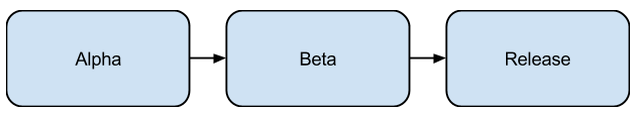
\includegraphics[width= 0.8 \textwidth]{pictures/Versions.png}
				\end{figure}
			\end{column}%
		\end{columns}
	\end{center}
\end{frame}

\begin{frame}
	\begin{center}
		\frametitle{Testing access}
		\begin{columns} % align columns
			\begin{column}{.3\textwidth}
				Who have access to what
			\end{column}%
			\begin{column}{.80\textwidth}
				\begin{figure}[H]
					\centering
					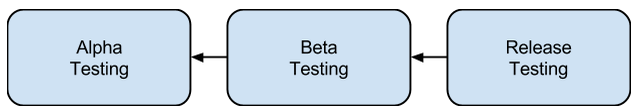
\includegraphics[width= 0.8 \textwidth]{pictures/Access.png}
				\end{figure}
			\end{column}%
		\end{columns}
	\end{center}
\end{frame}

\subsection{Google Analytics}
\begin{frame}
	\frametitle{Google Analytics}
\end{frame}

\begin{frame}
	\begin{center}
		\frametitle{Google Analytics}
		\begin{columns} % align columns
			\begin{column}{.3\textwidth}
				What it does
				\begin{itemize}
					\item Crash reports
					\item Statistics
				\end{itemize}
			\end{column}%
			\begin{column}{.3\textwidth}
				How we used it
				\begin{itemize}
					\item Transitioned away from it 
					\item Jenkins helped
				\end{itemize}
			\end{column}%
		\end{columns}
	\end{center}
\end{frame}

\subsection{Renaming}
\begin{frame}
	\frametitle{Renaming of Package-names}
\end{frame}

\begin{frame}
	\begin{center}
		\frametitle{Renaming process}
		\begin{columns} % align columns
			\begin{column}{.9\textwidth}
				\begin{tabular}{ll}
					\textbf{Old app package-names} & \textbf{New app package-names}\\ \hline \noalign{\vskip 2mm}
					launcher & launcher\\ \hline
					train & categorygame\\ \hline
					pictoadmin & categorymanager\\ \hline
					tortoise & lifestory\\ \hline
					oasis & administration\\ \hline
					parrot & pictoreader\\ \hline
					pictosearch & pictosearch\\ \hline
					pictocreator & pictocreator\\ \hline
					zebra & sequence\\ \hline
					cars & voicegame\\ \hline
					wombat & timer\\ \hline
					schedulestarter & ugeplan\\ \hline
				\end{tabular}
			\end{column}%
		\end{columns}
	\end{center}
\end{frame}